\begin{song}{title=\predtitle\centering Slavíci z Madridu \\\large Waldemar Matuška \vspace*{-0.3cm}}  %% sem se napíše jméno songu a autor
\begin{centerjustified}

\refren[1]
	Na\elipsa\dots\,na na\elipsa\dots

\phantom{.}

\begin{minipage}{0.65\textwidth}
\sloka
	^{Ami\z}Nebe je modrý a ^{E\z}zlatý, ^{E\z}bílá sluneční ^{Ami\z}záře,\:\:

	^{Ami\z}horko a sváteční ^{E\z}šaty, ^{E\z}vřava a zpocený ^{Ami\z}tváře.

	^{Ami\z}Vím,~co se bude ^{E}dít, ^{E\z}býk už se v ohradě ^{Ami\z}vzpíná,

	^{Ami\z}kdo~chce, ten může ^{E\z}jít, ^{E\z}já~si dám sklenici ^{Ami\z}vína.
\end{minipage}
\begin{minipage}{0.1\textwidth}
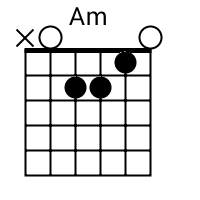
\includegraphics[width=3cm]{../Akordy/am}
\end{minipage}

\phantom{.}

\begin{minipage}{0.65\textwidth}
\refren[2]
	^{Dmi\z}Žízeň je veliká, ^{Ami\z}život mi utíká,

	^{E\z}nechte mě příjemně ^{Ami\z}snít,

	^{Dmi\z}ve~stínu pod fíky ^{Ami\z}poslouchat slavíky,

	^{E\z}zpívat si s nima a ^{Ami\z}pít.\:\:\:\:\:
\end{minipage}
\begin{minipage}{0.1\textwidth}
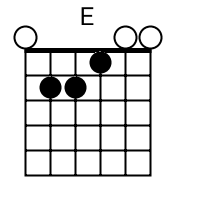
\includegraphics[width=3cm]{../Akordy/e}
\end{minipage}

\phantom{.}

\begin{minipage}{0.65\textwidth}
\sloka
	^{Ami\z}Ženy jsou krásný a ^{E\z}cudný, ^{E\z}mnohá se ve mně ^{Ami\z}zhlídla,

	^{Ami\z}oči~jako dvě ^{E\z}studny, ^{E\z}vlasy jak havraní ^{Ami\z}křídla.

	^{Ami\z}Dobře vím, co znamená ^{E}pád ^{E}do nástrah dívčího ^{Ami\z}klína,

	^{Ami\z}někdo má pletky ^{E\:}rád, ^{E}já si dám sklenici ^{Ami\z}vína.
\end{minipage}
\begin{minipage}{0.1\textwidth}
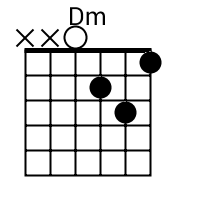
\includegraphics[width=3cm]{../Akordy/dm}
\end{minipage}

\phantom{.}

\refren[2]

\sloka
	^{Ami\z}Nebe je modrý a ^{E\z}zlatý, ^{E\z}ženy krásný a ^{Ami\z}cudný,

	^{Ami\z}mantily, sváteční ^{E\z}šaty, ^{E\z}oči jako dvě ^{Ami\z}studny.

	^{Ami\z}Zmoudřel jsem stranou od ^{E\z}lidí, ^{E\z}jsem jak ta zahrada ^{Ami\z}stinná,

	^{Ami\z}kdo~chce, ať mi ^{E\z}závidí, ^{E}já si dám sklenici ^{Ami\z}vína.\:

\refren[2]

\refren[1]

\end{centerjustified}
\setcounter{Slokočet}{0}
\end{song}
\begin{figure}[h]
\predtitle\centering
\end{figure}
